{\bf [40 points] Hidden Markov Models}\\

% In this question, we will explore Hidden Markov Models (HMM) and their use for genome annotation.    

\vspace{10pt} 

\textbf{Warm-Up}

\begin{figure}    
\begin{center} 
\tikzset{every picture/.style={line width=0.75pt}} %set default line width to 0.75pt        

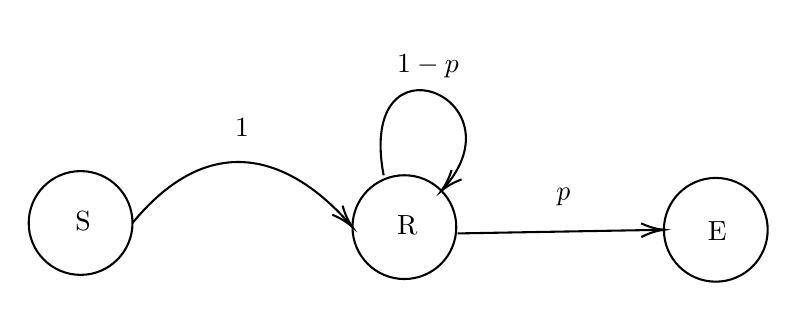
\begin{tikzpicture}[x=0.75pt,y=0.75pt,yscale=-1,xscale=1]
%uncomment if require: \path (0,131); %set diagram left start at 0, and has height of 131

%Shape: Circle [id:dp15981385446810636] 
\draw   (0,90) .. controls (0,76.19) and (11.19,65) .. (25,65) .. controls (38.81,65) and (50,76.19) .. (50,90) .. controls (50,103.81) and (38.81,115) .. (25,115) .. controls (11.19,115) and (0,103.81) .. (0,90) -- cycle ;
%Shape: Circle [id:dp1237743857732696] 
\draw   (156,92) .. controls (156,78.19) and (167.19,67) .. (181,67) .. controls (194.81,67) and (206,78.19) .. (206,92) .. controls (206,105.81) and (194.81,117) .. (181,117) .. controls (167.19,117) and (156,105.81) .. (156,92) -- cycle ;
%Straight Lines [id:da9619895708032187] 
\draw    (206.64,95.03) -- (304.04,93.31) ;
\draw [shift={(306.04,93.28)}, rotate = 178.99] [color={rgb, 255:red, 0; green, 0; blue, 0 }  ][line width=0.75]    (10.93,-3.29) .. controls (6.95,-1.4) and (3.31,-0.3) .. (0,0) .. controls (3.31,0.3) and (6.95,1.4) .. (10.93,3.29)   ;
%Curve Lines [id:da16728085201381981] 
\draw    (171,67) .. controls (157.8,-3.6) and (239.02,29.34) .. (199.89,73.35) ;
\draw [shift={(198.67,74.68)}, rotate = 313.24] [color={rgb, 255:red, 0; green, 0; blue, 0 }  ][line width=0.75]    (10.93,-3.29) .. controls (6.95,-1.4) and (3.31,-0.3) .. (0,0) .. controls (3.31,0.3) and (6.95,1.4) .. (10.93,3.29)   ;
%Curve Lines [id:da7636345097651801] 
\draw    (50,90) .. controls (99.34,30.17) and (143.82,78.23) .. (154.69,90.52) ;
\draw [shift={(156,92)}, rotate = 228.37] [color={rgb, 255:red, 0; green, 0; blue, 0 }  ][line width=0.75]    (10.93,-3.29) .. controls (6.95,-1.4) and (3.31,-0.3) .. (0,0) .. controls (3.31,0.3) and (6.95,1.4) .. (10.93,3.29)   ;
%Shape: Circle [id:dp9512059909455131] 
\draw   (306.04,93.28) .. controls (306.04,79.47) and (317.23,68.28) .. (331.04,68.28) .. controls (344.84,68.28) and (356.04,79.47) .. (356.04,93.28) .. controls (356.04,107.08) and (344.84,118.28) .. (331.04,118.28) .. controls (317.23,118.28) and (306.04,107.08) .. (306.04,93.28) -- cycle ;

% Text Node
\draw (252.53,72.17) node [anchor=north west][inner sep=0.75pt]  [rotate=-356.48] [align=left] {$\displaystyle p$};
% Text Node
\draw (176,7.4) node [anchor=north west][inner sep=0.75pt]    {$1-p$};
% Text Node
\draw (98,38.4) node [anchor=north west][inner sep=0.75pt]    {$1$};
% Text Node
\draw (21,83) node [anchor=north west][inner sep=0.75pt]   [align=left] {S};
% Text Node
\draw (325.72,88) node [anchor=north west][inner sep=0.75pt]   [align=left] {E};
% Text Node
\draw (176,85) node [anchor=north west][inner sep=0.75pt]   [align=left] {R};

\end{tikzpicture}
\label{HMM-prob1a}
\caption{Random Genome HMM}
\end{center}
\end{figure}

\begin{enumerate}

\item Consider the state transition diagram for the very simple HMM shown in Figure \ref{HMM-prob1a}. The state $S$ is a silent start state, and the state $E$ is a silent end state. The state $R$, which stands for \textit{random}, emits nucleotides with the following probabilities: 

\begin{center}
\begin{tabular}{|c|c|}
\hline
nucleotide& emission probability\\
\hline
A& 0.15 \\
C& 0.35 \\
G& 0.35 \\ 
T& 0.15 \\ 
\hline
\end{tabular}
\end{center}

The human genome is approximately 3.2 billion base pairs long. Suppose we generate a genome using the HMM in Figure \ref{HMM-prob1a}. Find the value of $p$ such that the expected length of this random genome is equal to the size of the human genome.

%%%%%%%%%%%%%%%%%%
\begin{solution}

\end{solution}
%%%%%%%%%%%%%%%%%%

\item Find the expected GC content of the genome generated in the previous part (write the answer as a percentage). 

%%%%%%%%%%%%%%%%%%
\begin{solution}

\end{solution}
%%%%%%%%%%%%%%%%%%

\clearpage

\textbf{Supervised Learning with HMMs}

\item  Consider the problem of supervised learning using HMMs. Specifically, we are given a set of $n$ observation sequences $O^{(i)} = o_1^{(i)}, \dots, o_{T_i}^{(i)}$ drawn from an alphabet set $O$, along with state annotation data $Q^{(i)} = q_1^{(i)}, \dots, q_{T_i}^{(i)}, (i=1, \dots, n),$ from a set of possible states $Q$. Here $T_i$ is the length of the $i$-th observation. Show that the maximum likelihood estimates for the HMM are 
\begin{align*} 
\hat{a}_{st} &= \frac{\sum_{i=1}^n \sum_{j=2}^{T_i} \mathbb{I} \left \{ q_{j-1}^{(i)} = s, q_j^{(i)} = t \right \} }{\sum_{i=1}^n \sum_{j=2}^{T_i} \sum_{t' \in Q} \mathbb{I} \left \{ q_{j-1}^{(i)} = s, q_j^{(i)} = t' \right \}},
\end{align*}
and 
\begin{align*}
\hat{e}_{s}(b) &= \frac{\sum_{i=1}^n \sum_{j=1}^{T_i} \mathbb{I} \left \{ q_{j}^{(i)} = s, o_j^{(i)} = b \right \} }{\sum_{i=1}^n \sum_{j=1}^{T_i} \sum_{b' \in O} \mathbb{I} \left \{ q_{j}^{(i)} = s, o_j^{(i)} = b' \right \}}.
\end{align*}
Here, $\mathbb I$ is the indicator function, which takes value $1$ when its argument is true and $0$ otherwise. 

%%%%%%%%%%%%%%%%%%
\begin{solution}

\end{solution}
%%%%%%%%%%%%%%%%%%

\vspace{10pt}
 

\textbf{HMMs Application}



% \item Coiled coils feature a repeated pattern every seven positions, shaped by the structural demands of the coiled coil formation. Consider building a HMM that make use of this repeated pattern to recognize which sequences are involved in coiled coils. You have labeled training data that includes a set of coiled coil sequences where you know 1) the start and the end positions of the coiled coil region 2) the seven positions involved in the pattern. Design a HMM and determine which method should you use to calculate the transition and emission probabilities.
CpG islands are DNA regions rich in cytosine (C) and guanine (G) nucleotides, commonly associated with gene promoter regions and regulation. Suppose you want to build a Hidden Markov Model (HMM) to recognize CpG islands within genomic DNA sequences.

\item Design a simple Hidden Markov Model to model genomic sequences for CpG island detection. Using a graphical illustration of your HMM design and clearly define the hidden states and the possible observations.

\begin{solution}

\end{solution}

% \item Suppose you have trained the above HMM and you want to know the location of the coiled coil region in a test sequence that is known to contain a coiled coil. List two methods that you could use to label the data and explain how do they work?

\item After training your HMM, you receive an unlabeled genomic DNA sequence. Describe two methods you could use to identify and locate CpG islands within this sequence. Briefly explain how each method works.
\begin{solution}

\end{solution}

% \item If all coiled coils have the repeated patterns. But the patterns are somewhat different in coiled coils that participate in 4-helix bundles and coiled coil pairs. Consider constructing separate HMMs (with the same topology but different parameters) to recognize sequences involved in this 2 patterns. Given two sets of unlabeled sequences that containing coiled coil sequences that form 4-helix bundles and coiled coil pairs separately. What method would you use to determine transition and emission probabilities and why?
\item Consider now that you have two separate biological conditions, e.g. healthy vs. diseased tissues, each potentially having different distributions of CpG islands. You wish to construct two HMMs, one per condition, from unlabeled sequences. What algorithm should you use to estimate the transition and emission probabilities for each model and why?
\begin{solution}

\end{solution}

\item Suppose you have trained the above 2 HMMs. You wish to determine if a new given unlabeled genomic sequence is more likely to originate from healthy or diseased tissue. What method would you use to do this?
\begin{solution}

\end{solution}

\end{enumerate}